\section{Structure of computations in \rdtlifsnns}
\label{ch:struct}

When working with neural networks a fundamental question is how well they are able to approximate functions. Towards that end the following theorem was proved in~\cite{nguyen2025timespikeunderstandingrepresentational}.

\begin{theorem}\label{thm:approx-snn-constant}
  Let \(f\) be a continuous function on a compact set \(Ω⊂ℝ^{n_0}\). For all \(ε>0\), there exists a d.t. LIF-SNN \(Φ\) with direct encoding, membrane potential output, \(L=2\) and \(T=1\) such that
  \[ \norm{(R(Φ)-f)|_{Ω}}_{∞}≤ε\]
  Moreover, if \(f\) is \(Γ\)-Lipschitz, then \(Φ\) can be chosen with width parameter \(n=(n_1,n_2)\) given by
  \begin{align*}
   n_1 &=\left(\max\left\{\left\lceil \frac{\operatorname{diam}_∞(Ω)}{ε}Γ \right\rceil,1\right\}+1\right)n_0, \\
   n_2 &=\max\left\{\left\lceil \frac{\operatorname{diam}_∞(Ω)}{ε}Γ \right\rceil^{n_0},1\right\}.
  \end{align*}
\end{theorem}

\begin{figure}[h!]
  \begin{subfigure}[t]{0.45\textwidth}
    \centering
    
\begin{tikzpicture}
  \begin{axis}[
    axis lines=middle,
    xmin=0, xmax=5,
    ymin=0, ymax=5,
    xtick={0, 1, 2, 3, 4},
    ytick={0, 1, 2, 3, 4},
    domain=0:5,
    samples=200,
    thick,
    legend pos=north west,
    width=\textwidth,
    height=6cm,
    legend style={legend cell align=left},
    ]
    \addplot[thick, red, dashdotdotted]{floor(x)+0.5};
    \addlegendentry{$ε=0.5$}
    \addplot[thick, purple, dashed]{floor(x*2)/2+0.25};
    \addlegendentry{$ε=0.25$}
    \addplot[blue]{x};
  \end{axis}
\end{tikzpicture}

    \caption{A \dtlifsnn approximating the identity}
    \label{fig:id-approx-by-dtlifsnn}
  \end{subfigure}
  \hfill
  \begin{subfigure}[t]{0.55\textwidth}
    \centering
    
\begin{tikzpicture}
  \begin{axis}[
    axis lines=middle,
    xmin=0, xmax=pi,
    ymin=0, ymax=1.2,
    xtick={0, pi/2, pi},
    xticklabels={$0$, $\frac{\pi}{2}$, $\pi$},
    ytick={0, 1},
    domain=0:pi,
    samples=200,
    thick,
    legend pos=north west,
    width=\textwidth,
    height=6cm,
    legend style={legend cell align=left},
    ]
    \addplot[thick, red, dashdotdotted]{(-cos(deg(floor(x*2+1)/2))+cos(deg(floor(x*2)/2)))*2};
    \addlegendentry{$ε=0.25$} % ε≈0.5*(1/2) (since sin(x)≈x for x≪1)
    \addplot[thick, purple, dashed]{(-cos(deg(floor(x*5+1)/5))+cos(deg(floor(x*5)/5)))*5};
    \addlegendentry{$ε=0.1$} % ε≈0.5*(1/5) (since sin(x)≈x for x≪1)
    \addplot[blue]{sin(deg(x))};
  \end{axis}
\end{tikzpicture}

    \caption{\Dtlifsnns approximating a sinus wave}
    \label{fig:sin-approx-by-dtlifsnn}
  \end{subfigure}
\end{figure}

The proof of~\cref{thm:approx-snn-constant} first shows that a continuous function can be arbitrarily approximated by step functions, in particular by step functions constant on hypercubes in \(Ω\).
Then a \dtlifsnn is constructed by using the first layer to partition the input space along hyperplanes into cubes and the second layer to assign values to the hypercubes.

While quite simple, this construction does not use the unique feature of \dtlifsnns/\rdtlifsnns, the ability of neurons to accumulate state over time. It therefore needs quite a lot more neurons than actually needed for many functions with (almost) linear segments, like a sinus wave. E.g. in~\cref{fig:sin-approx-by-dtlifsnn} a neuron is needed for every constant region of the graphs in the first and second layer each.

We will now show a more efficient construction for \rdtlifsnn using the fact that \rdtlifsnn can quite efficiently approximate linear segments. The general intuition behind it is to use piece-wise linear functions to approximate continuously differentiable functions and then construct a \rdtlifsnn approximating the piece-wise linear function by discretizing the input dimensions into spike trains in the first layer that are consumed by groups of neurons in the second layer, one group for each almost linear segment.

To state our theorem we first need to define the notions of “modulus of uniform continuity” and “generalized inverse of a modulus of uniform continuity” and proof some simple properties:

%TODO: quote def?
\begin{definition}
  Let \(M,N\) be metric spaces. A modulus of uniform continuity of a uniformly continuous function \(f:M→N\) is a function \(ω:[0,∞]→[0,∞]\), such that it vanishes at \(0\), i.e. \(\lim_{x→0}ω(x)=0\), and
  \[ ∀_{x,y∈M}d_N(f(x),f(y))≤ω(d_M(x,y)). \]
  The generalized inverse of \(ω\) is defined as
  \[ω^{†}(s)≔\inf\{t∈[0,∞]\mid ω(t)>s\}.\]
\end{definition}

\begin{lemma}\label{lem:inverse-cont-mod}
  Let \(ω:[0,∞]→[0,∞]\) be a modulus of uniform continuity of a uniformly continuous function \(f:M→N\), where \(M,N\) are metric spaces.

  We have the following properties
  \begin{enumerate}
  \item \(∀_{x,y∈M,s∈[0,∞]}d_M(x,y)≤ω^{†}(s)⇒d_N(f(x),f(y))≤s\).
  \item \(∀_{s∈[0,∞]}s=0⇔w^{†}(s)=0\).
  \end{enumerate}
\end{lemma}

\begin{proof}\phantom{}

  \begin{enumerate}
  \item Let \(x,y∈M\) and \(s∈[0,∞]\) be given such that \(d_M(x,y)≤ω^{†}(s)\). By definition of \(ω^{†}\), this means \(ω(d_M(x,y))≤s\). Since \(ω\) is a modulus of uniform continuity of \(f\), we have \(d_N(f(x),f(y))≤ω(d_M(x,y))\) and therefore overall \(d_N(f(x),f(y))≤s\).
  \item Since \(ω\) is a modulus of uniform continuity, it is by definition continuous at \(0\). Let us choose an arbitrary sequence \((t_n)_{n∈ℕ}\) with \(t_n→0\). Then \(ω(t_n)→0\) and therefore \(ω^{†}(0)≤\inf_{n∈ℕ}t_n=0\).

  Is on the other hand \(ω^{†}(s)=0\), then there is a sequence \((t_n)_{n∈ℕ}\) with \(t_n→0\) and therefore \(ω(t_n)→0\). By definition of \(ω^{†}(s)\), we have \(ω(t_n)>s\), so we get \(s=0\).
  \end{enumerate}
\end{proof}


% CANCELLED: In the end, we will see that we can in fact approximate any continuous function like this, by using mollification to extract an continuously differentiable approximation of the function.

% DONE: motivation (previous theorem + previous lower bound example), insatisfactory since d.t. SNN. have somewhat linear structure

% CANCELLED: extend to continuously differentiable functions apart from lebesgue-zero sets (where they are still continuous?)
% DONE: differentiable, but defined on compact subset of euclidean space???
%
% DONE: use generalized inverse of the modulus of continuity

Let us now state our theorem:

% CANCELLED: demand differentiability only for Ω°
\begin{theorem}\label{thm:approx-snn}
  Let \(f∈𝒞^0(C,ℝ^m)\) be defined on a half-open cube \(C≠∅\), such that \(f\mid_{C°}∈𝒞^1(C°,ℝ^m)\) is continuously differentiable with bounded differential, i.e. \(\norm{d(f|_{C°})}_{∞,2}<∞\). For all \(ε,μ,ν>0\), \(ε=μ+ν\), there exists a \rdtlifsnn \(Φ\) with \(L=2\) and
  \begin{align*}
   T   &= (K(μ)+1)T_r(ν)+2 \\
   n_1 &= n+1 \\
   n_2 &= K(μ)^n(n+1)+3
  \end{align*}
  such that
  \[ \norm{R(Φ)|_C-f}_{∞,2}≤ε.\]
  Where we use 
  \begin{align*}
   T_r&≔T_r(ν)≔\max\left(2,\left\lceil \sqrt{n}\frac{\operatorname{diam}_{∞}(C)}{K}\frac{\norm{d(f|_{C°})}_{∞,2}}{ν} \right\rceil\right), \\
   K&≔K(μ)≔ \min_{\substack{ξ,θ>0\\ξθ=μ}}\left\{\left\lceil \frac{\operatorname{diam}_∞(C)}{\frac{2}{\sqrt{n}}\min(ω^{†}(ξ) ,θ)} \right\rceil\right\}.
  \end{align*} %TODO: if ω^{†}=∞, then K=0?
  Here \(ω^{†}\) is the generalized inverse of a modulus of uniform continuity with regard to \(\norm{·}_2\) of the total derivative \(d(f|_{C°})\). \(d(f|_{C°})\) is uniformly continuous since it is bounded.
  Since \(ξ≠0\), we have \(ω^{†}(ξ)>0\) by~\cref{lem:inverse-cont-mod}. Further there are \(ξ,θ\) such that the minimum in the definition of \(K^n\) is obtained, since we the minimum is taken over the set of natural numbers, so \(K\) is well-defined. Moreover \(T_r\) is well-defined, since \(C≠0\) and therefore \(\operatorname{diam}_{∞}(C)≠0\) and \(K≠0\).
\end{theorem}

\begin{remark}
  In our construction \(μ\) and \(ν\) determine whether to optimize the number of neurons or the number of time-steps. As we see later, \(K^n\) corresponds to the number of subcubes we will split \(C\) into such that \(f\) is almost linear on each of them. From the definition it is clear that \(K\) and therefore the number of neurons only depend on \(f\) through \(ω^{†}(ξ)\), which is essentially a measure of how strongly the slope of \(f\) is changing and therefore into how many subcubes we need to split \(C\) to get sufficiently almost affine linear regions of \(f\).

  We will further see that \(T_r\) corresponds to the number of constant intervals with which we approximate \(f\) on the almost affine linear regions. It is therefore to be expected that \(T_r\) depends on the width \(\frac{\operatorname{diam}_{∞}(C)}{K}\) of the subcubes and the maximal slope \(\norm{d(f|_{C°})}_{∞,2}\).
\end{remark}
\begin{figure}[!ht]
  \centering
  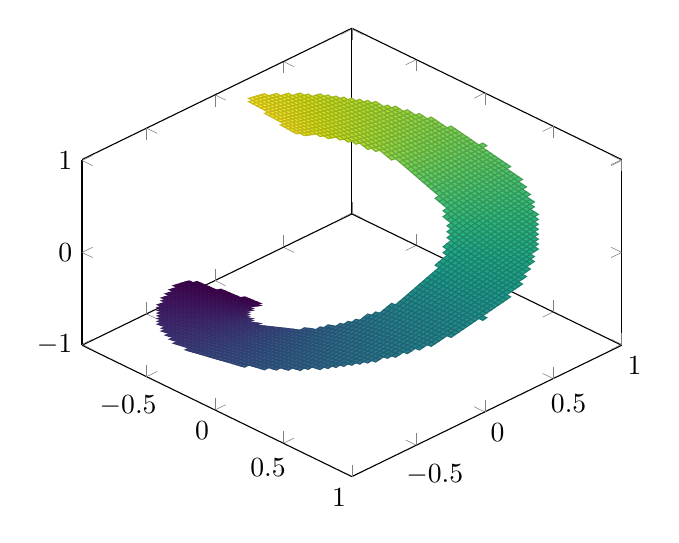
\begin{tikzpicture}
  \begin{axis}[title=,
    unbounded coords=jump,
    colormap/viridis,
    view={45}{45},
    ]
    \addplot3 [surf,domain=-1:1, samples=70] {(abs(atan2(y,x)) < deg(pi-0.2) && x^2+y^2 >= 0.25 && x^2+y^2 <= 1) ? atan2(y,x)/200 : nan};
  \end{axis}
\end{tikzpicture} 

  \caption{A spiral staircase function}
  \label{fig:ch03-spiral-staircase}
\end{figure}

\begin{remark}
  \cref{thm:approx-snn} cannot be generalized to arbitrary input spaces like compact sets: Consider a spiral staircase function like shown in~\cref{fig:ch03-spiral-staircase} defined on a compact set \(Ω≔\{(r\cos(φ),r\sin(φ))\mid 0.5≤r≤1,\ \abs{φ-π}≥0.2\}\). Such a function is clearly continuous and continuously differentiable on its interior \(Ω°\), such that in particular the differential is bounded, \(\norm{d(f|_{Ω°})}_{∞,2}<∞\).

  For our construction of the SNN we now need an encompassing half-open rectangle of \(Ω\), let e.g. \(C=[0,2)^2\). Now in~\cref{lem:approx-by-lin} we will partition \(C\) into sub-cubes, such that \(f\) is almost linear on those  w%TODO
  
  We need the half-open cube \(C\) with \(Ω⊂C⊂U\) to correctly choose \(T_r\) and \(K\): Suppose we regard the function \(f:((0,1) ∪ (2,3))→ℝ\), \(x↦χ_{[0,1]}(x)\). This function is certainly continuously differentiable, in particular, all derivatives are zero. In our construction of the \rdtlifsnn we use a cube in the input space as our canvas,
  %TODO
  Suppose, \(K\) would depend on the modulus of uniform continuity of \(df\) on \(U\) and \(T_r\) on \(\norm{df|_U}_{∞,2}\), without the a half-open cube \(C\) with \(Ω⊂C⊂U\)
\end{remark}

\begin{remark}
If \(f∈𝒞^1(U,ℝ^m)\) is given with \(∅≠U⊂ℝ^n\) and a compact subset \(Ω⊂ℝ^n\), we can extend \(f|_{Ω}\) to a function \(df∈𝒞^1(ℝ^n,ℝ^m)\): There is a partition of one \(φ_1,φ_2∈𝒞^{∞}(ℝ^n)\) subordinate to \(U\) and \(ℝ^n∖Ω\). We get \(φ_1|_{Ω}=1\) and therefore \((φ_1f)|_{Ω}=f|_{Ω}\). \(f'≔φ_1f\) is further clearly \(𝒞^1(U,ℝ^m)\).
% \item We would like to only demand differentiability on \(Ω°\), … %TODO

%TODO ↓
  % We would like to only demand differentiability on \(Ω°\), but the theorem would not be true anymore. Imagine the function \(f(x)=χ_{[0,1]}\) with \(Ω=[0,1]∪[2,3]\). Clearly, \(f|_{[0,1]∪[2,3]}\) is continuous and \(f|_{(0,1)∪(2,3)}∈𝒞^1(ℝ)\). But on the other hand a half-open cube around \(Ω\) at least needs to include \((1,2)\) and would need to have
\end{remark}


\begin{remark}%TODO
If \(f∈𝒞^1(U,ℝ^m)\) is given with \(∅≠U⊂ℝ^n\) and a compact \(Ω⊂ℝ^n\), but with no half-open cube \(C\) such that \(Ω⊂\overline{C}⊂U\), we can extend \(f|_{Ω}\) to a function \(df∈𝒞^1(ℝ^n,ℝ^m)\): There is a partition of one \(φ_1,φ_2∈𝒞^{∞}(ℝ^n)\) subordinate to \(U\) and \(ℝ^n∖Ω\). We get \(φ_1|_{Ω}=1\) and therefore \((φ_1f)|_{Ω}=f|_{Ω}\). \(f'≔φ_1f\) is further clearly \(𝒞^1(U,ℝ^m)\).
% \item We would like to only demand differentiability on \(Ω°\), … %TODO

%TODO ↓
  % We would like to only demand differentiability on \(Ω°\), but the theorem would not be true anymore. Imagine the function \(f(x)=χ_{[0,1]}\) with \(Ω=[0,1]∪[2,3]\). Clearly, \(f|_{[0,1]∪[2,3]}\) is continuous and \(f|_{(0,1)∪(2,3)}∈𝒞^1(ℝ)\). But on the other hand a half-open cube around \(Ω\) at least needs to include \((1,2)\) and would need to have
\end{remark}


%TODO: what about \dtlifsnn?

%TODO: remove?, minimal
\begin{comment}
%TODO
\begin{lemma}\label{lem:smallest-cube}
  Let \(Ω⊂ℝ^n\) be compact. Then there exists a half-open cube \(C\) with width \(\operatorname{diam}_∞(Ω)\) such that \(Ω⊂\overline{C}\).
\end{lemma}

%TODO: we later use ⟦y,z⦆ instead of ⟦a,b⦆; unify notation
\begin{proof}[\proofofref{lem:smallest-cube}]
  We can first define \(x≔(\inf_{x∈Ω} x_i)_{i∈[n]}∈ℝ^n\) since \(Ω\) is compact. We further define \(y≔x+\operatorname{diam}_∞(Ω)·𝟙_n\). We now have \(C≔⟦x,y⦆\). Suppose now a point \(z∈Ω∖\overline{C}\) exists. By definition of \(x\), we have \(x≤z\). By definition of \(C\) we further get \(z\nleq y\), and therefore \(y_i<z_i\) for an \(i∈[n]\) by definition of \(C\). But this means \(\norm{x-z}_∞>\operatorname{diam}_∞(Ω)\).
\end{proof}
\end{comment}

\begin{comment}
\begin{lemma}\label{lem:uniform-cont-≤}
  Let \(M\) be a normed vector space and \(N\) be a metric space. Let \(f:M→N\) be uniformly continuous with modulus \(δ\). We then have for every \(ε>0\):
  \[ ∀_{x,y∈M}(\norm{x-y}_M≤δ(ε)⇒d_N(x,y)≤ε). \]
\end{lemma}

\begin{proof}
  Let \(ε>0\) with modulus \(δ(ε)\), as well as \(x∈M\) be given. Since \(f\) is uniformly continuous with modulus \(δ(ε)\), we have \(f(B_{δ}(x))⊂B_{ε}(f(x))\). Since \(f\) is in particular continuous, we get
  \[ f(\overline{B}_{δ}(x))=f(\overline{B_{δ}(x)})⊂\overline{f(B_{δ}(x))}⊂\overline{B}_{ε}(f(x)) \]
  We need to use the fact that \(M\) is a normed vector space in the first equality to get \(\overline{B}_{δ}(x)=\overline{B_{δ}(x)}\).
\end{proof}
\end{comment}

% DONE: differentiable, but defined on compact subset of euclidean space???
% TODO: quote formulation?
% DONE: instead of fixing \(ε^{t}\), get supremum of
% TODO: why K≠0?
% CANCELLED: only demand differentiability on C°

We first proof that continuous differentiable functions with uniform continuous differential can be efficiently approximated by piece-wise linear function. Compare e.g.~\cref{fig:sin-approx-sinus-linear} to~\cref{fig:sin-approx-by-dtlifsnn}

\begin{figure}[h!]
  \centering
  \begin{minipage}{0.55\textwidth}
    \centering
    \begin{tikzpicture}
  \begin{axis}[
    axis lines=middle,
    xmin=0, xmax=pi,
    ymin=0, ymax=1.3,
    xtick={0, pi/2, pi},
    xticklabels={$0$, $\frac{\pi}{2}$, $\pi$},
    ytick={0, 1},
    domain=0:pi,
    samples=200,
    thick,
    legend pos=north west,
    width=\textwidth,
    height=6cm,
    legend style={legend cell align=left},
    declare function={
      myapproxSin(\len) = sin(deg(floor(x/\len)*\len+\len/2))+
                                       (x-(floor(x/\len)*\len+\len/2))*cos(deg(floor(x/\len)*\len+\len/2));
    },
    ]
    \addplot[blue, forget plot]{sin(deg(x))};
    \addplot[thick, red, dashed]{myapproxSin(0.62)}; % 0.62 ≈ π/5
    \addlegendentry{$ε=0.25$} % n_2(0.25) = ceil(sqrt(2)·π)=5; 0.6≈3.14/5

    \addplot[thick, green, dashdotdotted]{myapproxSin(1.571)}; % 1.571 ≈ π/2
    \addlegendentry{$ε=1$} %n_2(1) = ceil(π/sqrt(2))=2
  \end{axis}
\end{tikzpicture}

    \caption{Piece-wise affine linear functions approximating the sinus}
  \end{minipage}
  \label{fig:sin-approx-sinus-linear}
\end{figure}


\begin{lemma}\label{lem:approx-by-lin}
  Let \(f∈𝒞^0(C,ℝ^m)\) be a continuous function defined on half-open cube \(C\), such that \(f\mid_{C°}∈𝒞^1(C°,ℝ^m)\) is continuously differentiable and \(d(f|_{C°})\) is uniformly continuous. Let further \(K(μ)\) be defined as in~\cref{thm:approx-snn}.

  For every \(μ>0\) we can compose \(C\) into \(K^n≔K(μ)^n\) half-open subcubes \((C^{(j)})_{j∈[K^n]}\) such that affine linear functions \(g^{(j)}:C^{(j)}→ℝ^m\) exist with  \(\norm{d(g^{(j)})}_{∞,2}≤\norm{df}_{∞,2}\) and \(\norm{f-g}_{∞,2}<μ\), where \(g≔\sum_{i=1}^mg^{(j)}χ_{C^{(j)}}\).
\end{lemma}

% TODO: remark about why we are using 2-norm

% DONE: fix issue with C^(j) s not completely fitting in open \sqrt{2}δ(μ) balls due to closed part of C^(j)
% CANCELLED: F might not be defined at c^(j), since \(Ω≠\overline{C}\)

\begin{proof}[\proofofref{lem:approx-by-lin}]
  Let \(μ>0\) be given. Let \(ω\) be a modulus of uniform continuity of \(df\mid_{C°}\).
  We will now partition \(C\) in \(K^n\) half-open subcubes with \(K\) defined as in~\cref{thm:approx-snn}.
  Let \(ξ,Θ\) be given, such that the minium is attained. Then the subcubes have width \(w≔\frac{\operatorname{diam}_∞(C)}{K}≤\frac{2}{\sqrt{n}}\min(ω^{†}(ξ),θ)\).

  Let us further define \(g^{(j)}:C^{(j)}→ℝ^m\) by \(g^{(j)}(x)≔f(c^{(j)})+df_{c^{(j)}}(x-c^{(j)})\) where \(c^{(j)}\) is the center of \(C^{(j)}\), so in particular for all  \(x∈C^{(j)}\)
  \begin{equation}\label{eq:4}
  \norm{x-c^{(j)}}_2=\sqrt{\sum_{i=1}^n\abs{(x-c^{(j)})_i}^2}≤\frac{w}{2}\sqrt{n}≤\min(ω^{†}(ξ),θ).
  \end{equation}
  Now by definition of \(g^{(j)}\) we already have \(\norm{d(g^{(j)})}_{∞,2}=\norm{df_{c^{(j)}}}≤\norm{df}_{∞,2}\).

  It suffices now to show \(\norm{f|_{C^{(j)}}-g^{(j)}}_∞<μ\). Let \(x∈C^{(j)}\) and \(h(t)≔f(t(x-c^{(j)})+c^{(j)})\). We then have
  \[h'(t)=(df_{(x-c^{(j)})t+c^{(j)}}∘d(t↦t(x-c^{(j)})+c^{(j)})_t)(1)=df_{(x-c^{(j)})t+c^{(j)}}(x-c^{(j)}).\]
  We obtain by the fundamental theorem of calculus:
  \begin{align*}
    \norm{f(x)-g^{(j)}(x)}_2 &= \norm{f(x)-f(c^{(j)})-df_{c^{(j)}}(x-c^{(j)})}_2 \\
          &= \norm{h(1)-h(0)-df_{c^{(j)}}(x-c^{(j)})}_2 \\
          &= \norm{\int_0^1df_{(x-c^{(j)})t+c^{(j)}}(x-c^{(j)})dt-df_{c^{(j)}}(x-c^{(j)})}_2
  \end{align*}
  Due to the generalized Minkowski-Inequality we can move the norm inside the integral:
  %MAYBE: ref for gen. Minkowski-Ineq?
  \begin{align*}
    &≤ \int_0^1\norm{df_{(x-c^{(j)})t+c^{(j)}}(x-c^{(j)})-df_{c^{(j)}}(x-c^{(j)})}_2dt \\
    &= \int_0^1\norm{(df_{(x-c^{(j)})t+c^{(j)}}-df_{c^{(j)}})(x-c^{(j)})}_2dt \\
    &≤ \int_0^1\norm{df_{(x-c^{(j)})t+c^{(j)}}-df_{c^{(j)}}}_2\norm{x-c^{(j)}}_2dt \\
    &≤ \int_0^1ξ\norm{x-c^{(j)}}_2dt \\
    &= ξ\norm{x-c^{(j)}}_2 \\
    &≤ ξθ \\
    &= μ
  \end{align*}
  In the fourth step we use \(\norm{df_{(x-c^{(j)})t+c^{(j)}}-df_{c^{(j)}}}≤ξ\), which holds due to \(∀_{t∈[0,1]}(x-c^{(j)})t+c^{(j)}∈C^{(j)}\),~\eqref{eq:4} and~\cref{lem:inverse-cont-mod}.
  %CANCELLED: proof for cont. extension
\end{proof}
%DONE change notation of c_i to sth clearly not meant component

\begin{proof}[\proofofref{thm:approx-snn}.]
  Let there be \(ε,μ,ν>0\) with \(ε=μ+ν\).
  %DONE: clarify notation ⟦y,z⦆ (line or proper subspace)
  By~\cref{lem:approx-by-lin} we have a composition \(K^n\) of \(C\) into half-open subcubes \((C^{(j)})_{i=1..K^n}\) and linear functions \(g^{(j)}:C^{(j)}→ℝ^m\), such that \(\norm{d(g^{(j)})}_{∞,2}≤\norm{df}_{∞,2}\) and \(\norm{f-g}_∞<μ\) for \(g≔\sum_{i=1}^mg^{(j)}χ_{C^{(j)}}\). %CANCELLED: cont ext?

  We will now define a \rdtlifsnn \(Φ\) with direct input encoding and membrane-potential outputs such that \(\norm{R(Φ)|_C-g}_∞<ν\).

  Let us first set the basic parameters \(i^{[l]}(0)=0\), \(α^{[l]}=0\) and \(β^{[l]}=ϑ^{[l]}=1\) for all layers.

  \begin{figure}[h!]
    \centering
    \usetikzlibrary{positioning, chains, shapes.geometric, fit, shapes, arrows.meta, calc, backgrounds}

\begin{tikzpicture}[
    >=LaTeX, % Use default LaTeX arrows
    % Styles 
    node/.style={ % Input or output node
        circle,
        minimum width=2.25em,
        draw,
        fill=gray!10,
        thick,
        font=\scriptsize
    },
    group/.style={
        rectangle,
        rounded corners=1mm,
        draw,
        thick
    }, 
    innerNode/.style={
        circle,
        minimum width=0.3em,
        inner sep=0pt,
        draw,
        fill=gray!10,
        thick
    },
    arrow/.style={
        -latex,
        thick
    },
    backprop/.style={ % Backpropagation arrows
        arrow,
        dashed,
        gray
    }
]
    
    % Input
    \foreach \x in {1,...,2}
        \draw node at (0, -\x*1.25 - 0.625) [node] (first_\x) {$x_\x$};
    \draw node at (0, -5*1.25 + 0.625) [node] (first_n) {$x_n$};
    \path (first_2) -- (first_n) node[pos=0.5, scale=2] {$\vdots$};
    
    % Hidden 1
    \foreach \x in {1,...,2}
        \node at (2.5, -\x*1.25) [node] (second_\x){$\x$};
    \draw node at (2.5, -4*1.25) [node] (second_n) {$n$};
    \path (second_2) -- (second_n) node[pos=0.5, scale=2] {$\vdots$};
    \draw node at (2.5, -5*1.25) [node] (second_a1) {$a_1$};

    % Hidden 2
    \newcommand{\nodeGroup}[2]{
      \foreach \x in {1,...,2}
      \node at (5, #2-\x*0.25) [innerNode] (#1_\x){};
      \node at (5, #2-4*0.25) [innerNode] (#1_om){};
      \path (#1_2) -- (#1_om) node[pos=0.5, scale=0.5] {$\vdots$};
      \node[group, dashed, fit=(#1_1) (#1_om)] (#1) {};
    }
    \nodeGroup{third_1}{-0.25}
    \nodeGroup{third_kn}{-2.4}
    \path (third_1) -- (third_kn) node[pos=0.5, scale=2] {$\vdots$};

    \draw node at (5, -4.5) [node] (third_a2) {$a_2$};
    \draw node at (5, -4.5-1*1.1) [node] (third_c1) {$c_1$};
    \draw node at (5, -4.5-2*1.1) [node] (third_c2) {$c_2$};
    
    % Output
    \foreach \x in {1,...,2}
        \node at (7.5, -\x*1.25 - 0.625) [node] (fourth_\x){$y_\x$};
    \draw node at (7.5, -5*1.25 + 0.625) [node] (fourth_m) {$y_m$};
    \path (fourth_2) -- (fourth_m) node[pos=0.5, scale=2] {$\vdots$};

    % Input -> hidden 1
    \foreach \i in {1,2,n}
        \draw [arrow] (first_\i) to (second_\i);

    % A1 -> hidden 1
    \foreach \i in {1,2,n}
        \draw [arrow, bend left=40, color=gray] (second_a1) to (second_\i);

    % C1/C2/A2 -> hidden 2
    \foreach \i in {c1,c2,a2}
        \foreach \j in {1,kn}
            \draw [arrow, bend left=40, color=gray] (third_\i) to (third_\j);
    
    % hidden 1 -> hidden 2
    \foreach \i in {1,2,n}
        \foreach \j in {1,kn}
        \draw [arrow] (second_\i) to (third_\j);

    \draw [arrow, bend left=20] (third_kn) to (third_1);

    % hidden 2 -> Output
    \foreach \i in {1,kn}
        \foreach \j in {1,2,m}
        \draw [arrow] (third_\i) to (fourth_\j);

    % loops
    \path[arrow, color=gray] (second_a1) edge[loop left] ();
    \path[arrow, color=gray] (third_a2) edge[loop left] ();
    \path[arrow, color=gray] (third_c1) edge[loop left] ();
    \path[arrow, color=gray] (third_c2) edge[loop left] ();
    \path[arrow] (third_1) edge[loop left] ();
    \path[arrow] (third_kn) edge[loop left] ();

    % Layer Labels
    \node[above=0.25cm of first_1] (xlabel) {Input};
    \node[above=0.25cm of second_1] (h1label) {First hidden layer};
    \node[above=0.25cm of third_1] (h2label) {Second hidden layer};
    \node[above=0.25cm of fourth_1] (ylabel) {Output};
\end{tikzpicture}

% adapted from https://github.com/fraserlove/nntikz/tree/main

    \caption{Structure of the whole network}
    \label{fig:ch03-whole-network}
  \end{figure}

  \begin{figure}[h!]
    \centering
    \usetikzlibrary{positioning, chains, shapes.geometric, fit, shapes, arrows.meta, calc, backgrounds}

\begin{tikzpicture}[
    >=LaTeX, % Use default LaTeX arrows
    % Styles 
    node/.style={ % Input or output node
        circle,
        minimum width=2.25em,
        inner sep=0.5pt,
        draw,
        fill=gray!10,
        thick,
        font=\scriptsize
    },
    group/.style={
        rectangle,
        rounded corners=1mm,
        draw,
        thick
    }, 
    innerNode/.style={
        circle,
        minimum width=0.3em,
        inner sep=0pt,
        draw,
        fill=gray!10,
        thick
    },
    arrow/.style={
        -latex,
        thick
    },
    backprop/.style={ % Backpropagation arrows
        arrow,
        dashed,
        gray
    }
]
    
    % Input
    \foreach \x in {1,...,1}
        \draw node at (0, -\x*1.25 - 1.25) [node] (first_\x) {$x_\x$};
    \draw node at (0, -3*1.25 -1.25) [node] (first_n) {$x_n$};
    \path (first_1) -- (first_n) node[pos=0.5, scale=2] {$\vdots$};
    
    % Hidden 1
    \foreach \x in {1,...,1}
        \node at (2.5, -0.625-\x*1.25) [node] (second_\x){$\x$};
    \draw node at (2.5, -0.625-3*1.25) [node] (second_n) {$n$};
    \path (second_1) -- (second_n) node[pos=0.5, scale=2] {$\vdots$};
    \draw node at (2.5, -0.625-4*1.25) [node] (second_a1) {$a_1$};

    % Hidden 2
    \node at (5, 0.25-1.1) [node] (third_1_1){$ι_j(1)$};
    \node at (5, 0.25-2*1.1-0.75) [node] (third_1_n){$ι_j(n)$};
    \path (third_1_1) -- (third_1_n) node[pos=0.5, scale=2] {$\vdots$};
    \node at (5, 0.25-3*1.1-0.75) [node] (third_1_om){$ω_j$};
    \node[group, dashed, fit=(third_1_1) (third_1_om)] (third_1) {};

    \draw node at (5, -6) [node] (third_a2) {$a_2$};
    \draw node at (5, -6-1*1.1) [node] (third_c1) {$c_1$};
    \draw node at (5, -6-2*1.1) [node] (third_c2) {$c_2$};

    \path (third_1) -- (third_a2) node[pos=0.5, scale=2] (third_vdots) {$\vdots$};
    
    % Output
    \foreach \x in {1,...,2}
        \node at (7.5, -\x*1.25 - 0.625) [node] (fourth_\x){$y_\x$};
    \draw node at (7.5, -5*1.25 + 0.625) [node] (fourth_m) {$y_m$};
    \path (fourth_2) -- (fourth_m) node[pos=0.5, scale=2] {$\vdots$};

    % Input -> hidden 1
    \foreach \i in {1,n}
        \draw [arrow] (first_\i) to (second_\i);

    % A1 -> hidden 1
    \foreach \i in {1,n}
        \draw [arrow, bend left=40, color=gray] (second_a1) to (second_\i);

    % C1/C2/A2 -> hidden 2
    \foreach \i in {c1,c2}
        \foreach \j in {1,n}
            \draw [arrow, bend left=40, color=gray] (third_\i) to (third_1_\j);
    \draw [arrow, bend left=40, color=gray] (third_a2) to (third_1_om);

    % connect group to itself
    \foreach \i in {1,n}
    \foreach \j in {om} {
      \draw [arrow, bend left=60] (third_1_\j) to (third_1_\i);
      \draw [arrow, bend right=30] (third_1_\i) to (third_1_\j);
    }

    % group to other groups
    \draw [arrow, bend left=30] (4.9, -4.9) to (third_1_om);
    \draw [arrow, bend right=20] (third_1_om) to (4.95, -4.7);
    
    % hidden 1 -> hidden 2
    \foreach \i in {1,n}
        \draw [arrow] (second_\i) to (third_1_\i);

    % hidden 2 -> Output
    \foreach \i in {1}
        \foreach \j in {1,2,m}
        \draw [arrow] (third_\i) to (fourth_\j);

    % loops
    \path[arrow, color=gray] (second_a1) edge[loop left] ();
    \path[arrow, color=gray] (third_a2) edge[loop left] ();
    \path[arrow, color=gray] (third_c1) edge[loop left] ();
    \path[arrow, color=gray] (third_c2) edge[loop left] ();
    \path[arrow] (third_1_om) edge[loop left] ();

    % Layer Labels
    \node[above=0.25cm of first_1] (xlabel) {Input};
    \node[above=0.25cm of second_1] (h1label) {First hidden layer};
    \node[above=0.25cm of third_1] (h2label) {Second hidden layer};
    \node[above=0.25cm of fourth_1] (ylabel) {Output};
\end{tikzpicture}

% adapted from https://github.com/fraserlove/nntikz/tree/main

    \caption{Structure of the network, focused on the \(j\)-th group of the second layer}
    \label{fig:ch03-group-network}
  \end{figure}

  The intuitive idea for the construction of the network is the following: We have five phases. We define
  \begin{gather*}
    T_1≔\rangeI{1}{KT_r},\qquad T_2≔\{KT_r\}, \qquad T_3≔\{KT_r+1\},\\
    T_4≔\{KT_r+2\},\qquad T_5≔\rangeI{KT_r+3}{T}.
  \end{gather*}
  For ease of notation, will also use \(T_2,T_3,T_4\) as if they were numbers.

  The first layer is only active during the first phase, \(T_1\). It is composed of \(n+1\) neurons, where the first \(n\) neuron convert the input vector regarding its position in \(C\) into spike trains. The last neuron, the “alarm clock”, shuts down the first layer after \(T_1\) ends.

  The second layer only accumulates state without spike during \(T_1∖T_2\). Then during \(T_2∪T_3∪T_4\) it is decided in which region \(C^{(j)}\) the input \(x\) is located. Further during \(T_4∪T_5\) the location in \(C^{(j)}\) is encoded through spikes.

  For each region \(C^{(j)}\) we have \(n+1\)-neurons in the second layer. Each of the first \(n\) neurons encodes a commponent of the linear part of \(g^{(j)}\). They are also used to inform the \(n+1\)-th neuron of the group if the \(x\) has at least as big as the base point of \(C^{(j)}\). The \(n+1\)-th deactivates all other neurons of regions with smaller base point and encodes the constant part of \(g^{(j)}\). The last \(3\) neurons act as “clock neurons” enabling and disabling the other ones.

  % In the second layer we have \(m+1\)-neurons for each affine linear region \(C^{(j)}\). Each of the first \(m\) neurons encodes the linear part of a component of the output vector. The last, additional neuron acts as an activator to the specific region by recursively enabling the other neurons of this region and disabling all regions with smaller base point (that would otherwise be enabled).
  
  %TODO: properly label/name and ref graphics
  \tikzstyle{descript} = [text = black,align=center, minimum height=1.8cm, align=center, outer sep=0pt,font = \footnotesize]
\tikzstyle{activity} =[align=center,outer sep=1pt]
\definecolor{ColorOne}{named}{MidnightBlue}

% #1 = color
% #2 = left coordinate
% #3 = right coordinate
\newcommand{\FillRegion}[3]{%
  \fill[#1] (#2) -- (#3) -- ($(#3)+(0,1)$) -- ($(#2)+(0,1)$);
}

\newenvironment{timeline}{
\begin{tikzpicture}[very thick, black]
  \small
  
  \coordinate (O) at (0,0);
  \coordinate (T2-1) at (3,0);
  \coordinate (T2) at (5,0);
  \coordinate (T3) at (7,0);
  \coordinate (T4) at (9,0);
  \coordinate (T4+1) at (11,0);
  \coordinate (T) at (14,0);
  
  \FillRegion{ColorOne!10!white}{O}{T2-1}

  \fill[
    pattern={Lines[angle=45,distance=6pt,line width=3pt, xshift=4.5pt]},
    pattern color=ColorOne!20!white
  ] (T2-1) rectangle ($(T2)+(0,1)$);
  \fill[
    pattern={Lines[angle=45,distance=6pt,line width=3pt]},
    pattern color=ColorOne!10!white
  ] (T2-1) rectangle ($(T2)+(0,1)$);

  \FillRegion{ColorOne!30!white}{T2}{T3}
  \FillRegion{ColorOne!40!white}{T3}{T4}
  \FillRegion{ColorOne!50!white}{T4}{T}
  % \FillRegion{ColorOne!60!white}{T4+1}{T}
  
  \draw ($(O)!0.5!(T2-1)+(0,0.5)$) node[activity] {$T_1$};
  \draw ($(T2-1)!0.5!(T2)+(0,0.5)$) node[activity] {$T_2$};
  \draw ($(T2)!0.5!(T3)+(0,0.5)$) node[activity] {$T_3$};
  \draw ($(T3)!0.5!(T4)+(0,0.5)$) node[activity] {$T_4$};
  \draw ($(T4)!0.5!(T)+(0,0.5)$) node[activity] {$T_5$};

  %% Timeline
  \draw[dotted] (O) -- (T2-1);
  \draw (T2-1) -- (T4+1);
  \draw[dotted] (T4+1) -- (T);
  \draw[->] (T) -- ($(T)+(0.5,0)$);

  %% Ticks
  \foreach \pos/\labeltext in {
    O/$0$,
    T2-1/$T_2-1$,
    T2/$T_2$,
    T3/$T_3$,
    T4/$T_4$,
    T4+1/$T_4+1$,
    T/$T$
  }{
    % Draw tick
    \draw (\pos) ++(0,3pt) -- ++(0,-6pt);
    % Add label below
    \node[below=4pt, anchor=north] at (\pos) {\labeltext};
  }
}{\end{tikzpicture}}

% adapted from https://www.overleaf.com/project/68b326ec3dceb466ee45cc28

% #1 = coordinate
% #2 = label
\NewDocumentCommand{\SpikeOut}{O{} O{} O{} m}{%
        \draw[->,thick,color=black,#1] ($(#4)+(0,0)$) -- ($(#4)+(0,1.5)$) node [above=0pt,align=center,black] {#2} node[midway, sloped, yshift=7pt] {\color{gray} #3};
}
\NewDocumentCommand{\SpikeIn}{O{} O{} O{} m}{%
        \draw[<-,thick,color=black,#1] ($(#4)+(0,0)$) -- ($(#4)+(0,1.5)$) node [above=0pt,align=center,black]  {#2} node[pos=0,anchor=north] {\rotatebox{90}{#3}};
}

% #1 = number of holes/number of points-1
% #2 = size of circles
% #3 = coordinate 1
% #4 = coordinate 2
\newcommand{\dotsT}[4]{
  \foreach \i in {0,...,#1} {
    \coordinate (P\i) at ($ (#3)!{\i/#1}!(#4) $);
    \fill (P\i) circle (#2); % draw point
  }
}

% https://tex.stackexchange.com/questions/604337/comparing-node-coordinates-in-tikz
\makeatletter
\newcommand{\gettikzxy}[3]{%
  \tikz@scan@one@point\pgfutil@firstofone#1\relax
  \edef#2{\the\pgf@x}%
  \edef#3{\the\pgf@y}%
}
\makeatother

% #1 = coordinate 1
% #2 = coordinate 2
\newcommand{\dotsBtSp}[3][15]{
  \dotsT{#1}{0.5pt}{$(#2)+(0,1.3)$}{$(#3)+(0,1.3)$};
  \dotsT{#1}{0.5pt}{$(#2)+(0,0.2)$}{$(#3)+(0,0.2)$};
}

\newcommand{\drawSpikeOutFrom}[1]{
  \gettikzxy{(#1)}{\px}{\py}
  \foreach \name in {T2,T3,T4,T4+1} {
    \gettikzxy{(\name)}{\qx}{\qy}

    \ifdimcomp{\qx}{>=}{\px}{
        \SpikeOut{$(\name)-(0.3,0)$}{};
    }{}
  }
  \dotsBtSp{$(T4+1)-(0.1,0)$}{$(T)+(-0.5,0)$};
  \SpikeOut{$(T)+(-0.3,0)$}{};
}

\NewDocumentCommand{\SpikeOutAt}{O{} O{} O{} m}{%
  \SpikeOut[#1][#2][#3]{$(#4)-(0.3,0)$};
}


  \begin{figure}[h!]
    \centering
    \begin{subfigure}{\textwidth}
      \centering
      \begin{timeline}
        \SpikeOutAt{$(T2)$}
        \SpikeOutAt{$(T3)$}
        \SpikeOutAt{$(T4)$}
        \SpikeOutAt{$(T4+1)$}
        \dotsBtSp{$(T4+1)-(0.1,0)$}{$(T)+(-0.5,0)$}
        \SpikeOutAt{$(T)$}
      \end{timeline}
      
      \caption{$a_1$}
      \label{fig:timeline-a1}
    \end{subfigure}

    \begin{subfigure}{\textwidth}
      \centering

      \begin{timeline}
        \SpikeIn[][$x_i$]{$(O)+(0.3,0)$}
        \SpikeOut[dashed]{$(O)+(0.6,0)$}{}
        \dotsBtSp{$(O)+(0.8,0)$}{$(T2)+(-0.8,0)$}
        % TODO:
        \SpikeIn[][$x_i$]{$(T2)+(-0.6,0)$}
        \SpikeOut[dashed]{$(T2)+(-0.3,0)$}

        \SpikeIn[][$x_i$]{$(T3)+(-1.8,0)$}
        \SpikeIn[][$s_{a_1}^{[1]}$]{$(T3)+(-1.3,0)$}

        \SpikeIn[][$x_i$]{$(T4)+(-1.8,0)$}
        \SpikeIn[][$s_{a_1}^{[1]}$]{$(T4)+(-1.3,0)$}

        \SpikeIn[][$x_i$]{$(T4+1)+(-1.8,0)$}
        \SpikeIn[][$s_{a_1}^{[1]}$]{$(T4+1)+(-1.3,0)$}

        \dotsBtSp{$(T4+1)-(1.1,0)$}{$(T)+(-1,0)$}

        \SpikeIn[][$x_i$]{$(T)+(-0.8,0)$}
        \SpikeIn[][$s_{a_1}^{[1]}$]{$(T)+(-0.3,0)$}
      \end{timeline}
      
      \caption{$i$}
      \label{fig:timeline-i}
    \end{subfigure}
    \caption{Timelines of first layer neurons}
    \label{fig:timeline-first-layer}
  \end{figure}
  

  \begin{figure}[h!]
    \centering
    \begin{subfigure}{\textwidth}
      \centering

      \begin{timeline}
        \SpikeOutAt{$(T2-1)$}
      \end{timeline}
      
      \caption{$c_1$}
      \label{fig:timeline-c_1}
    \end{subfigure}

    \begin{subfigure}{\textwidth}
      \centering

      \begin{timeline}
        \SpikeOutAt{$(T2)$}
      \end{timeline}
      
      \caption{$c_2$}
      \label{fig:timeline-c2}
    \end{subfigure}

    \begin{subfigure}{\textwidth}
      \centering

      \begin{timeline}
        \SpikeOutAt{$(T4)$}
        \SpikeOutAt{$(T4+1)$}
        \dotsBtSp{$(T4+1)-(0.1,0)$}{$(T)+(-0.5,0)$}
        \SpikeOutAt{$(T)$}
      \end{timeline}
      \caption{$a_2$}
      \label{fig:timeline-a2}
    \end{subfigure}

    \begin{subfigure}{\textwidth}
      \centering

      \begin{timeline}
        \SpikeIn[double][$\sum_{i∈[n]}s^{[2]}_{ι_j(i)}$][]{$(T3)-(1.7,0)$}
        \SpikeOut[dashed][][$x^{C^{(j)}}{≤}x$]{$(T3)-(0.3,0)$}
        \SpikeIn[double][$r_s(q^{(j)})$][]{$(T4)-(1.5,0)$}
        \SpikeOut[dashed][][$x{∈}C^{(j)}$]{$(T4)-(0.2,0)$}

        \SpikeIn[][$s_{a_2}^{[1]}$]{$(T4+1)+(-1.7,0)$}

        \dotsBtSp{$(T4+1)-(1.5,0)$}{$(T)+(-0.5,0)$}

        \SpikeIn[][$s_{a_2}^{[1]}$]{$(T)+(-0.3,0)$}
      \end{timeline}
      \caption{$ω_j$}
      \label{fig:timeline-ommega}
    \end{subfigure}

    \begin{subfigure}{\textwidth}
      \centering

      \begin{timeline}
        \SpikeIn[][$x_i$]{$(O)+(0.3,0)$}
        \dotsBtSp[12]{$(O)+(0.5,0)$}{$(T2)+(-2,0)$}
        \SpikeIn[][$x_i$]{$(T2)+(-1.8,0)$}
        \SpikeIn[][$s^{[2]}_{c_1}$]{$(T2)+(-1.3,0)$}
        \SpikeIn[][$s^{[2]}_{c_2}$]{$(T3)+(-1.7,0)$}
        \SpikeIn[double][$r_s(q^{(j)})$]{$(T4)+(-1.7,0)$}
        \SpikeIn[double][$r_s(q^{(j)})$]{$(T4+1)+(-1.7,0)$}

        \SpikeOut[dashed][][$x^{C^{(j)}}_i{≤}x_i$]{$(T2)+(-0.2,0)$}

        \SpikeOutAt[dashed]{$(T4+1)$}
        \dotsBtSp{$(T4+1)-(0.1,0)$}{$(T)+(-0.5,0)$}
        \SpikeOutAt[dashed]{$(T)$}
        % \draw [decorate,decoration={brace,amplitude=6pt}] ($(T4+1)+(-0.4,1.6)$) -- ($(T)+(-0.2,1.6)$) node[midway,above=6pt]{\small If \(x∈C_j\), };
      \end{timeline}
      \caption{$ι_j(i)$}
      \label{fig:timeline-iota_i}
    \end{subfigure}
    \caption{Timelines of second layer neurons}
    \label{fig:timeline-second-layer}
  \end{figure}

  To obtain the normalized location of a value in \(C\) we will often us
  \[ o_i(z)=\frac{z_i-x_i^C}{y_i^C-x_i^C} \]
  with \(i∈[n_1]\) in the following. 

  \begin{enumerate}
  \item \textbf{First layer}:
  We define the \textbf{\(i\)-th neuron} of the \(n\) neurons of the first layer by parameters
  \begin{equation}
    w=\frac{1}{y^C_i-x^C_i}e_i, \quad b=-\frac{x^C_i}{y^C_i-x^C_i}
    , \quad v=-e_{a_1},\quad u_0=0, \quad i_0=0.\tag{\(i\)}
  \end{equation}
  The \textbf{“alarm neuron”} of the first layer, with index \(a_1≔n+1\), is defined by:
  \begin{equation}
    w=0, \quad b=\frac{1}{T_2}, \quad v=e_{a_1}, \quad u_0=0, \quad i_0=0.\tag{\(a_1\)}
  \end{equation}

  % CANCELLED: check that proof works for x∈\(\overline{C}∖C\)

  % We further define the \(n+1\)-th neuron of the first layer by \(w=0\), \(b=\frac{1}{K-1}\), \(v=\)
  % By~\cref{lem:non-recursive-defs} we get

  % DONE: proof correct behaviour

  %DONE: a_2 is used wrongly
  %DONE: add timeline
  \item \textbf{Second layer}:
  Let us now construct the second layer in the following way: For each of the \(K^n\) subcubes in \(C\) we define \(n+1\) neurons like so: Let \(C^{(j)}=⟦x^{C^{(j)}},y^{C^{(j)}}⦆\) be one such subcube with position \(q^{(j)}∈([K-1]_0)^{n_1}\) in \(C\), i.e.
  \[∀_{i∈[n_1]}q^{(j)}_i=Ko_i(x^{C^{(j)}}).\]
  We will write \(ι_j(i)≔j(n+1)+i\) to index the first \(n\) neurons in the layer and \(ω_j≔(j+1)(n+1)\) to index the last neuron of each group.

  The \textbf{\(i\)-th neuron} of the first \(n\) neurons (of the \(j\)-th group), with index \(ι_j(i)\) in the second layer, has the parameters
  \begin{equation}
  \begin{gathered}
    w=e_i, \quad b=0, \quad v=T(e_{c_1}-2e_{c_2}+r(q^{(j)})), \\
    u_0=-q^{(j)}_iT_r-T+1, \quad i_0=0.
  \end{gathered}\tag{\(ι_j(i)\)}
  \end{equation}
  where “the switch” is
  \[ r(q)≔e_{ω_{j(q)}}-\sum_{\substack{q'∈([K-1]_0)^{n_1} \\ q<q'}}e_{ω_{j(q')}}. \]
  with the index \(j(q)\) of the subcube at position \(q\). We further define the applied variant
  \[ r_s(q;t)≔⟨r(q),s^{[2]}(t)⟩=s^{[2]}_{ω_{j(q)}}(t)-\sum_{\substack{q'∈([K-1]_0)^{n_1} \\ q<q'}}s^{[2]}_{ω_{j(q')}}(t). \]
  The \textbf{final neuron} of the group, with index \(ω_j\) in its layer, has the parameters
  \begin{equation}
  \begin{gathered}
    w=0, \quad b=0, \quad v=\frac{1}{n}\sum_{i=1}^ne_{ι_j(i)}-2e_{a_2}+r(q^{(j)}), \quad u_0=0, \quad i_0=0.
  \end{gathered}\tag{\(ω_j\)}
  \end{equation}
  We also define the two \textbf{“clock neurons”}, with index \(c_1≔(n+1)K^n+1\) and \(c_2≔(n+1)K^n+2\) with parameters:
  %TODO: T_2=1?
  \begin{equation}
  \begin{gathered}
    w=0, \quad b=b_{c_i}, \quad v=-(T-1)e_{c_i}, \quad u_0=0, \quad i_0=0.
  \end{gathered}\tag{\(c_1,c_2\)}
  \end{equation}
  where \(b_{c_1}=\frac{1}{T_2-1}\) and \(b_{c_2}=\frac{1}{T_2}\).
  We further define the \textbf{“alarm neuron”}, with index \(a_2≔(j+1)K^n(μ)+3\), by
  \begin{equation}
  \begin{gathered}
    w=0, \quad b=\frac{1}{T_4}, \quad v=e_{a_2}, \quad u_0=0, \quad i_0=0.
  \end{gathered}\tag{\(a_2\)}
  \end{equation}
  %DONE: use c_{-1}, c_0 and c_{1} and a (for alarm) for the first layer neuron.
  \item Output decoder:
    We further define the parameters of the output decoder by \(a_t=0\), for \(t≤T_3\) and otherwise \(a_t=1\). We further set \(b^{[L+1]}=0\) and
    \[ (W^{[L+1]})_{k,ι_j(i)}=d(g^{(j)})_k((y^{C^{(j)}}_i-x^{C^{(j)}}_i)\frac{1}{T_r}e_i) \] %TODO: remove parantheses?
    for \(k∈[m]\), \(j∈K^n\) and \(i∈[n]\). Here \(d(g^{(j)})\) is not only the total derivative, but also the linear part of \(g^{(j)}\), i.e. \(∀_{x∈C^{(j)}}g^{(j)}(x)=d(g^{(j)})(x-x^{C^{(j)}})+g(x^{C^{(j)}})\). We further set
    \[ (W^{[L+1]})_{k,ω_j}=g_k(x^{C^{(j)}}) \]
    for \(k∈[m]\) and \(j∈K^n\). We finally define \(W^{[L+1]}_{k,c_i}=0\) for \(i∈\{2..4\}\).
    %TODO: indices in correct order?
    %TODO: make easier to read
  \end{enumerate}

  We will now proof that this construction indeed approximates \(g\) well enough. It will be helpful to consider the following, by choice of \(i^{[l]},α^{[l]},β^{[l]},ϑ^{[l]}\), simplified equations:
  \begin{align*}
    i^{[l]}(t) & = W^{[l]}s^{[l-1]}(t)+V^{[l]}s^{[l]}(t-1) \\
    p^{[l]}(t) & = u^{[l]}(t-1)+i^{[l]}(t)+b^{[l]} \\
    s^{[l]}(t) & = H(p^{[l]}(t)-\oneV{n_l}) \\
    u^{[l]}(t) & = p^{[l]}(t)-s^{[l]}(t)
  \end{align*}
  and in particular by~\cref{lem:non-recursive-defs}
  \begin{align*}
   p^{[l]}(t) &= u^{[l]}(0)+\sum_{k=1}^t\left(i^{[l]}(t)+b^{[l]}\right)-\sum_{k=1}^{t-1}s^{[l]}(k).
  \end{align*}

  Let now \(s^{[0]}(t)=x∈C\). We will proof \(\norm{R(Φ)(x)-g(x)}_{∞,2}≤ν\) in steps, by first characterizing the behavior of the first layer:

  \begin{enumerate}
  \item Characterization of the “alarm neuron” \(a_1\):\\
  Let us first regard the neuron in the first layer: By choice of parameters we get:
  \begin{equation*}
   p^{[1]}_{a_1}(t) = \frac{t}{T_2}+\sum_{k=1}^ts^{[1]}_{a_1}(k-1)-\sum_{k=1}^{t-1}s^{[1]}_{a_1}(k) = \frac{t}{T_2}
  \end{equation*}
  So \(s^{[1]}_{a_1}(t)=1⇔t≥T_2\).
  \item Characterization of \(i\)-th neuron, \(i∈[n]\):\\
  We have
  \begin{align*}
   i^{[1]}_i(t)+b^{[1]}_i=\frac{x_i-x^C_i}{y^C_i-x^C_i}-s^{[1]}_{a_1}(t-1)=o_i(x)-s^{[1]}_{a_1}(t-1).
  \end{align*}
  So in particular
  \begin{align*}
   0≤i^{[1]}_i(t)+b^{[1]}_i=o_i(x)≤1
  \end{align*}
  for \(t∈T_1\), since \(x^C_i≤x_i<y_i^C\).
  Because further \(0≤u^{[1]}_i(0)=0<1\) we can use~\cref{lem:sum-spikes-slowly-through-time} with \(t_0≔0\) and \(t_{ω}≔T_2\) to obtain
  \begin{equation*}
  \left\lfloor T_2o_i(x) \right\rfloor =\left\lfloor u^{[1]}_i(0)+\sum_{t=1}^{T_2}(i^{[1]}_i(t)+b^{[1]}_i) \right\rfloor = \sum_{t=1}^{T_2}s^{[1]}_i(t).
  \end{equation*}
  
  We further have
  \begin{equation*}
   i^{[1]}_i(t)+b^{[1]}_i=o_i(x)-s^{[1]}_{a_1}(t-1)=o_i(x)-1<0
  \end{equation*}
  for \(t>T_2\), so we get
  \[p_i^{[1]}(t)=u_i^{[1]}(T_2)+\sum_{k=T_3}^t\left(i^{[1]}_i(k)+b^{[1]}_i\right)-\sum_{k=T_3}^{t-1}s^{[1]}(k) <1\]
  and therefore \(s_i^{[1]}(t)=0\) for \(t>T_2\).

  % So in particular
  % \begin{equation}\label{eq:3}
  % \left\lfloor T_2\frac{x_i-x^C_i}{y^C_i-x^C_i} \right\rfloor = \sum_{t=1}^{T_2}s^{[1]}_i(t) = \sum_{t=1}^Ts^{[1]}_i(t)
  % \end{equation}

  % The equation clearly also holds for \(x_i=y_i\).
  \end{enumerate}
  
  \noindent We will now continue with characterizing the second layer. We start with “clock neurons” and the “alarm” neuron:
  
  \begin{enumerate}
  \item Characterization of the “clock neurons”: \\
  In contrast to the alarm neuron of the first layer, the two “clock” neurons only fire once:
  \begin{equation*}
   p^{[2]}_{c_i}(t) = tb_{c_i}-(T-1)\sum_{k=1}^ts^{[2]}_{c_i}(k-1)-\sum_{k=1}^{t-1}s^{[2]}_{c_i}(k)=tb_{c_i}-T\sum_{k=1}^{t-1}s^{[2]}_{c_i}(k)
  \end{equation*}
  %DONE: proof t<3(T_2-1)
  Let us first consider \(c_1\): We clearly have \(p^{[2]}_{c_1}(t)<1\) for \(t<T_2-1\), but \(p^{[2]}_{c_1}(T_2-1)=1\).
  Since by definition \(K≥1\) and \(T_r≥2\), so \(T_2=KT_r≥2\), we have \(t≤T≤T(T_2-1)\). Therefore \(p^{[2]}_{c_1}(t)<1\) for \(t>T_2-1\) due to \(s^{[2]}_{c_1}(T_2-1)=1\). So \(∀_{t∈[T]}s^{[2]}_{c_1}(t)=χ_{\{T_2-1\}}(t)\).

  We similarly obtain \(∀_{t∈[T]}s^{[2]}_{c_2}(t)=χ_{T_2}(t)\).
  \item Characterization of the “alarm neuron”:\\
  Just like for \(a_1\), we also get \(s^{[1]}_{a_2}(t)=1⇔t≥T_4\).
  \end{enumerate}

  \noindent We now proof the behavior of the remaining neurons in the second layer step by step throughout the phases.
  \begin{enumerate}
  \item Phase 1 \\
  We will show \(∀_{i∈[n]}s^{[2]}_{ι_j(i)}(t)=0\) and \(s^{[2]}_{ω_j}(t)=0\) for all \(j∈[K^n]\) and \(t∈[T_2-1]_0\) by induction over \(t\). Let \(t=0\). We then get \(s^{[2]}_{ι_j(i)}(0)=s^{[2]}_{ω_j}(0)=0\) by definition.
  Let further \(1≤t≤T_2-1\). First notice that by induction hypothesis, we have \(∀_{i∈[n]}s^{[2]}_{ι_j(i)}(t')=0\) and \(r_s(q^{(j)};t')=0\) for \(t'<t\). It follows that
  \begin{align*}
   i^{[2]}_{ι_j(i)}(t')+b^{[2]}_{ι_j(i)}&=s^{[1]}_i(t')+T(s^{[2]}_{c_1}(t'-1)-2s^{[2]}_{c_2}(t'-1)+r_s(q^{(j)};t'-1))=s^{[1]}_i(t'), \\
   i^{[2]}_{ω_j}(t')+b^{[2]}_{ω_j}&=\frac{1}{n}\sum_{i=1}^ns^{[2]}_{ι_j(i)}(t'-1)-2s^{[2]}_{a_2}(t'-1)+r_s(q^{(j)};t'-1)=0.
  \end{align*}
  for all \(t'≤t\). Thus, we further get
  \begin{align*}%TODO: t' anstatt k
   p^{[2]}_{ι_j(i)}(t) &= -q^{(j)}_iT_r-T+1+\sum_{k=1}^ts^{[1]}_i(k)-\sum_{k=1}^{t-1}s^{[2]}_{ι_j(i)}(k)= -q^{(j)}_iT_r-T+1+\sum_{k=1}^ts^{[1]}_i(k),\\
   p^{[2]}_{ω_j}(t) &= \sum_{k=1}^t0-\sum_{k=1}^{t-1}s^{[2]}_{ω_j}(k) = 0.
  \end{align*}
   Since \(\sum_{k=1}^ts^{[1]}_i(k)≤T_2-1<T-1\) and \(s^{[2]}_{c_1}(t)=χ_{\{T_2-1\}}(t)\), we in particular get \(p^{[2]}_{ι_j(i)}(t)≤0\). So we have prooven \(∀_{i∈[n]}s^{[2]}_{ι_j(i)}(t)=0\), \(s^{[2]}_{ω_j}(t)=0\).
  \item Phase 2 \\
  Just as in phase 1, we have
  \begin{align*}
   i^{[2]}_{ω_j}(T_2)+b^{[2]}_{ω_j}&=\frac{1}{n}\sum_{i=1}^ns^{[2]}_{ι_j(i)}(T_2-1)-2s^{[2]}_{a_2}(T_2-1)+r_s(q^{(j)};T_2-1)=0.
  \end{align*}
  So we also get \(p^{[2]}_{ω_j}(T_2)=0\) and \(s^{[2]}_{ω_j}(T_2)=0\). It is different for \(ι_j(i)\) due to the dependence on \(c_1\). Let \(j∈[K^n]\) and \(i∈[n]\) be given. The neuron with index \(ι_j(i)\) fires exactly then at \(T_2\), if \(x_i≥x^{C^{(j)}}_i\):
  First notice that
  \begin{align*}
   i^{[2]}_{ι_j(i)}(T_2)+b^{[2]}_{ι_j(i)}&=s^{[1]}_i(T_2)+T(s^{[2]}_{c_1}(T_2-1)-2s^{[2]}_{c_2}(T_2-1)+r_s(q^{(j)};T_2-1))=s^{[1]}_i(T_2)+T,
  \end{align*}
  thus, we conclude that
  \begin{align*}
   p^{[2]}_{ι_j(i)}(T_2) &= p^{[2]}_{ι_j(i)}(T_2-1) + i^{[2]}_{ι_j(i)}(T_2)+b^{[2]}_{ι_j(i)} - s^{[2]}_{ι_j(i)}(T_2-1) \\
                         &= -q^{(j)}_iT_r+1+\sum_{k=1}^{T_2}s^{[1]}_i(k) \\
                         &= -q^{(j)}_iT_r+1+\left\lfloor T_2o_i(x) \right\rfloor
  \end{align*}
  holds using the characterization of layer 1. Therefore we have \(s^{[2]}_{ι_j(i)}(T_2)=1\) exactly if \(q^{(j)}_iT_r≤T_2o_i(x)\), which is equivalent to \(\frac{q^{(j)}_i}{K}(y^C_i-x^C_i)+x_i^C≤x_i\) by definition of \(o_i\). Further \(\frac{q^{(j)}_i}{K}(y^C_i-x^C_i)+x_i^C\) is equal to \(x^{C^{(j)}}\) by definition of \(q^{(j)}\). So \(s^{[2]}_{ι_j(i)}(T_2)=1\) holds exactly if \(x^{C^{(j)}}_i≤x_i\).
  \item Phase 3 \\
  The “Activator neuron” \(ω_j\) fires at \(T_3\) if and only if \(x^{C^{(j)}}≤x\): First notice
  \begin{align*}
   i^{[2]}_{ω_j}(T_3)+b^{[2]}_{ω_j}&=\frac{1}{n}\sum_{i=1}^ns^{[2]}_{ι_j(i)}(T_2)-2s^{[2]}_{a_2}(T_2)+r_s(q^{(j)};T_2)=\frac{1}{n}\sum_{i=1}^ns^{[2]}_{ι_j(i)}(T_2).
  \end{align*}
  from which we derive
  \begin{align*}
   p^{[2]}_{ω_j}(T_3) &= p^{[2]}_{ω_j}(T_2) + i^{[2]}_{ω_j}(T_3)+b^{[2]}_{ω_j} - s^{[2]}_{ω_j}(T_2) = \frac{1}{n}\sum_{i=1}^ns^{[2]}_{ι_j(i)}(T_2).
  \end{align*}
  So \(0≤p^{[2]}_{ω_j}(T_3)≤1\) and we get \(p^{[2]}_{ω_j}(T_3)=1\), as well as \(s^{[2]}_{ω_j}(T_3)=1\) exactly if \(∀_{i∈[n_1]}x^{C^{(j)}}_i≤x_i\), so if \(x^{C^{(j)}}≤x\).

  Let further \(i∈[n_1]\). We get
  \begin{align*}
   i^{[2]}_{ι_j(i)}(T_3)+b^{[2]}_{ι_j(i)}&=s^{[1]}_i(T_3)+T(s^{[2]}_{c_1}(T_2)-2s^{[2]}_{c_2}(T_2)+r_s(q^{(j)};T_2))=-2T
  \end{align*}
  and therefore
  \begin{align*}
    p^{[2]}_{ι_j(i)}(T_3) &= p^{[2]}_{ι_j(i)}(T_2)+i^{[2]}_{ι_j(i)}(T_3)+b^{[2]}_{ι_j(i)} - s^{[2]}_{ι_j(i)}(T_2) \\
                          &= -q^{(j)}_iT_r+1+\left\lfloor T_2o_i(x) \right\rfloor-2T - s^{[2]}_{ι_j(i)}(T_2).
  \end{align*}
  So \(p^{[2]}_{ι_j(i)}(T_3)≤-T\) and \(s^{[2]}_{ι_j(i)}(T_3)=0\), since \(\left\lfloor T_2o_i(x) \right\rfloor≤T_2≤T-1\).
  \item Phase 4 \\
  Let \(i∈[n]\). The neuron \(ι_j(i)\) stays inactive at \(T_4\), since
  \begin{align*}
   i^{[2]}_{ι_j(i)}(T_4)+b^{[2]}_{ι_j(i)}&=s^{[1]}_i(T_4)+T(s^{[2]}_{c_1}(T_3)-2s^{[2]}_{c_2}(T_3)+r_s(q^{(j)};T_3))=Tr_s(q^{(j)};T_3)
  \end{align*}
  and hence
  \begin{align*}
    p^{[2]}_{ι_j(i)}(T_4) &= p^{[2]}_{ι_j(i)}(T_3)+i^{[2]}_{ι_j(i)}(T_4)+b^{[2]}_{ι_j(i)} - s^{[2]}_{ι_j(i)}(T_3) \\
                        &= p^{[2]}_{ι_j(i)}(T_3)+Tr_s(q^{(j)};T_3).
  \end{align*}
  Since \(p^{[2]}_{ι_j(i)}(T_3)≤-T\), we conclude \(p^{[2]}_{ι_j(i)}(T_4)≤0\) and \(s^{[2]}_{ι_j(i)}(T_4)=0\).

  Further the “activator neuron” \(ω_j\) fires at \(T_4\) exactly if \(x∈C^{(j)}\): First notice
  \begin{align*}
   i^{[2]}_{ω_j}(T_4)+b^{[2]}_{ω_j}&=\frac{1}{n}\sum_{i=1}^ns^{[2]}_{ι_j(i)}(T_3)-2s^{[2]}_{a_2}(T_3)+r_s(q^{(j)};T_3)=r_s(q^{(j)};T_3).
  \end{align*}
  So we get
  \begin{align*}
    p^{[2]}_{ω_j}(T_4) &= p^{[2]}_{ω_j}(T_3)+i^{[2]}_{ι_j(i)}(T_4)+b^{[2]}_{ι_j(i)} - s^{[2]}_{ι_j(i)}(T_3) \\
                       &= p^{[2]}_{ω_j}(T_3)+r_s(q^{(j)};T_3) - s^{[2]}_{ι_j(i)}(T_3). \\
  \end{align*}
  By definition of \(q\), \(q^{(j)}_i<q^{(j')}_i\) holds exactly if \(x^{C^{(j)}}_i<x^{C^{(j')}}_i\) holds for all \(i∈[n_1]\) and \(j,j'∈[K^n]\), so \(∀_{j,j'∈[K^n]}q^{(j)}<q^{(j')}⇔x^{C^{(j)}}<x^{C^{(j')}}\).
  We further have shown \(∀_{j'∈K^n}s^{[2]}_{ω_{j'}}(T_3)=1⇔x^{C^{(j')}}≤x\) before.
  \begin{align*}
  r_s(q^{(j)};T_3)&=s^{[2]}_{ω_j}(T_3)-\sum_{\substack{q'∈([K-1]_0)^{n_1} \\ q^{(j)}<q'}}s^{[2]}_{ω_{j(q')}}(T_3) \\
                  &=s^{[2]}_{ω_j}(T_3)-\sum_{\substack{j'∈[K^n] \\ x^{C^{(j)}}<x^{C^{(j')}}≤x}}1
  \end{align*}%TODO: n_1 vs n

  Now if \(x∈C^{(j)}\), i.e. \(x^{C^{(j)}}≤x<y^{C^{(j)}}\), then \(s^{[2]}_{ω_j}(T_3)=1\) and if there was a \(s^{[2]}_{ω_{j'}}(T_3)=1\) with \(x^{C^{(j)}}<x^{C^{(j')}}≤x\), we would further get \(x^{C^{(j)}}<x^{C^{(j(q'))}}<y^{C^{(j)}}\) due to \(x<y^{C^{(j)}}\). But this contradicts the construction of the subcubes \((C^{(j)})_{j∈[K^n]}\).
  
  We have also shown \(p^{[2]}_{ω_j}(T_3)=1\) and \(s^{[2]}_{ω_j}(T_3)=1\) for this case, so we can conclude \(p^{[2]}_{ω_j}(T_4)=1\) as well as \(s^{[2]}_{ω_j}(T_4)=1\).

  Now suppose \(x∉C^{(j)}\). Since we assumed \(x∈C\) and constructed the subcubes \((C^{(j)})_{j∈[K^n]}\) as a partition of \(C\), we have \(x∈C^{(j')}\), \(j≠j'\). Now if \(x^{C^{(j)}}<x^{C^{(j')}}\), then \(r_s(q^{(j)};T_3)≤0\). We further have \(p^{[2]}_{ω_j}(T_3)=1\) and \(s^{[2]}_{ω_j}(T_3)=1\) in this case and therefore \(p^{[2]}_{ω_j}(T_4)≤0\) and \(s^{[2]}_{ω_j}(T_4)=0\).

  Is on the other hand \(x^{C^{(j)}}≮x^{C^{(j')}}\), then there is a component \(i∈[n_1]\), such that \(x^{C^{(j')}}_i<x^{C^{(j)}}_i\) and therefore \(x_i<y^{C^{(j')}}_i≤x^{C^{(j)}}_i\). This implies \(x^{C^{(j)}}\nleq x\) and we also get \(r_s(q^{(j)};T_3)≤0\). We further have have \(p^{[2]}_{ω_j}(T_3)<1\) and \(s^{[2]}_{ω_j}(T_3)=0\) in this case and therefore \(p^{[2]}_{ω_j}(T_4)<1\) and \(s^{[2]}_{ω_j}(T_4)=0\).

  To summarize, we \(s^{[2]}_{ω_j}(T_4)=1\) exactly if \(x∈C^{(j)}\) just as we claimed, as well as \(p^{[2]}_{ω_j}(T_4)≤1\) in general.
  %DONE: more rigorous?
  \item Phase 5 \\
  The “activator neuron” \(ω_j\) is inactive during \(T_5\), since for \(t>T_4\)
  \begin{align*}
   i^{[2]}_{ω_j}(t)+b^{[2]}_{ω_j}&=\frac{1}{n}\sum_{i=1}^ns^{[2]}_{ι_j(i)}(t-1)-2s^{[2]}_{a_2}(t-1)+r_s(q^{(j)};t-1)≤0.
  \end{align*}
  and
  \begin{align*}
     p^{[2]}_{ω_j}(t) &= u^{[2]}_{ω_j}(T_4)+\sum_{k=T_4+1}^{t}\left(i^{[2]}_{ω_j}(k)+b^{[2]}_{ω_j}\right)-\sum_{k=T_4+1}^{t-1}s^{[2]}_{ω_j}(k) \\
                      &≤ u^{[2]}_{ω_j}(T_4). \\
  \end{align*}
  Further \(u^{[2]}_{ω_j}(T_4)<1\), since \(p^{[2]}_{ω_j}(T_4)≤1<2\). So \(∀_{t>T_4}s^{[2]}_{ω_j}(t)=0\). In particular the “switch” \(r_s(q^{(j)};t)=0\) is off for all \(j∈[K^n]\) and \(t>T_4\).
  
  Let \(i∈[n]\). During \(T_5\) the neuron \(ι_j(i)\) captures the position of \(x\) in \(C^{(j)}\) regarding the \(i\)-th dimension if \(x∈C^{(j)}\) and stays inactive otherwise.

  Let us first assume \(x∉C^{(j)}\). We have previously shown \(s^{[2]}_{ω_j}(T_4)=0\) and just now \(∀_{t>T_4}s^{[2]}_{ω_j}(t)=0\). So \(∀_{t≥T_4}r_s(q^{(j)};t)=0\) and therefore for all \(t>T_4\)
  \begin{align*}
   i^{[2]}_{ι_j(i)}(t)+b^{[2]}_{ι_j(i)}&=s^{[1]}_i(t)+T(s^{[2]}_{c_1}(t-1)-2s^{[2]}_{c_2}(t-1)+r_s(q^{(j)};t-1))≤0
  \end{align*}
  as well as
  \begin{align*}
    p^{[2]}_{ι_j(i)}(t) &= p^{[2]}_{ι_j(i)}(T_4)+\sum_{k=T_4+1}^t\left(i^{[2]}_{ι_j(i)}(k)+b^{[2]}_{ι_j(i)}-s^{[2]}_{ι_j(i)}(k-1)\right) \\
                        &= p^{[2]}_{ι_j(i)}(T_4)+\sum_{k=T_4+1}^t\left(i^{[2]}_{ι_j(i)}(k)+b^{[2]}_{ι_j(i)}-s^{[2]}_{ι_j(i)}(k-1)\right) \\
                      &≤p^{[2]}_{ι_j(i)}(T_4) \\
                      &≤0. \\
  \end{align*}
  So in particular \(∀_{t>T_4}s^{[2]}_{ι_j(i)}(t)=0\).

  Suppose now \(x∈C^{(j)}\).


  Let \(j\) be given with \(x∈C^{(j)}\). As we have seen before, we have \(r_s(q^{(j)};T_4)=1 \) and \(∀_{t>T_4}r_s(q^{(j)};t)=0\).
  We therefore get
  \begin{align*}
   i^{[2]}_{ι_j(i)}(T_4+1)+b^{[2]}_{ι_j(i)}&=s^{[1]}_i(T_4+1)+T(s^{[2]}_{c_1}(T_4)-2s^{[2]}_{c_2}(T_4)+r_s(q^{(j)};T_4)) = T
  \end{align*}
  and for all \(t>T_4+1\)
  \begin{align*}
    i_{ι_j(i)}^{[2]}(t)+b^{[2]}_{ι_j(i)}=&s^{[1]}_i(t)+T(s^{[2]}_{c_1}(t-1)-2s^{[2]}_{c_2}(t-1)+r_s(q^{(j)};t-1))=0.
  \end{align*}
    
  Using previous results and in particular \(s^{[2]}_{ι_j(i)}(T_2)=1⇔x^{C^{(j)}}_i≤x_i\), we obtain
  \begin{align*}
    p_{ι_j(i)}^{[2]}(T_4+1)&=p_{i_j(i)}^{[2]}(T_4)+i^{[2]}_{ι_j(i)}(T_4+1)+b^{[2]}_{ι_j(i)}-s^{[2]}_{ι_j(i)}(T_4) \\
                           &=p^{[2]}_{ι_j(i)}(T_3)+Tr_s(q^{(j)};T_3)+T \\
                           &=-q^{(j)}_iT_r+1+\left\lfloor T_2o_i(x) \right\rfloor-2T - s^{[2]}_{ι_j(i)}(T_2)+2T \\
                           &=-KT_ro_i(x^{C^{(j)}})+\left\lfloor KT_ro_i(x) \right\rfloor.
  \end{align*}
  We now have \(KT_ro_i(x^{C^{(j)}})≤KT_ro_i(x) \), since \(x^{C^{(j)}}_i≤x_i\), so \(p_{ι_j(i)}^{[2]}(T_4+1)≥0\).

  We further have 
  \[ o_i(y^{C^{(j)}})-o_i(x^{C^{(j)}})=\frac{y_i^{C^{(j)}}-x_i^{C^{(j)}}}{y_i^C-x_i^C}=\frac{1}{K}. \]
  and \(o_i(x)<o_i(y^{C^{(j)}})=o_i(x^{C^{(j)}})+\frac{1}{K}\) for all \(x∈C^{(j)}\). We can deduce
  \begin{align*}
    p_{ι_j(i)}^{[2]}(T_4+1) &=-KT_ro_i(x^{C^{(j)}})+\left\lfloor KT_ro_i(x) \right\rfloor \\
    &≤-KT_ro_i(x^{C^{(j)}})+KT_ro_i(y^{C^{(j)}}) \\
    &≤-KT_ro_i(x^{C^{(j)}})+T_r+KT_ro_i(x^{C^{(j)}}) \\
    &≤T_r.
  \end{align*}
  So we have shown
  \[ 0≤p_{ι_j(i)}^{[2]}(T_4+1)=u_{i_j(i)}^{[2]}(T_4)+i^{[2]}_{ι_j(i)}(T_4+1)+b^{[2]}_{ι_j(i)}≤T_r=T-(T_4+1). \]
  By~\autoref{lem:pos-input-pos-res-pos} we now get \(u^{[2]}_j(T_4+1)≥0\). We can therefore use~\autoref{lem:sum-spikes-decaying} with \(t_0≔T_4+1\), \(t_m≔T_4+1\) and \(t_ω≔T\), such that we obtain
  \begin{align*}
    \sum_{t=T_4+1}^Ts^{[2]}_{ι_{j(i)}}(t)&=\left\lfloor u^{[2]}_{ι_{j(i)}}(T_4)+i^{[2]}_{ι_{j(i)}}(T_4+1)+b^{[2]}_{ι_{j(i)}} \right\rfloor \\
                                         &=-KT_ro_i(x^{C^{(j)}})+\left\lfloor KT_ro_i(x) \right\rfloor.
  \end{align*}

  \end{enumerate}

  \noindent We have now reached the final step, where we will show that the spikes actually approximate \(g\). Let us consolidate our results. For \(j\) with \(x∈C^{(j)}\) we have
  \begin{align*}
    &\sum_{t=T_4}^Ts^{[2]}_{ι_{j(i)}}(t)=\sum_{t=T_4+1}^Ts^{[2]}_{ι_{j(i)}}(t)= -KT_ro_i(x^{C^{(j)}})+\left\lfloor KT_ro_i(x) \right\rfloor, \\
    &\sum_{t=T_4}^Ts^{[2]}_{ω_j}(t)=s^{[2]}_{ω_j}(T_4)=1.
  \end{align*}
  And therefore for all \(k∈[m]\) %TODO: split into parts
  \begin{align*}
   W^{[L+1]}_{k,ω_j}\sum_{t=T_4}^Ts^{[2]}_{ω_j}(t) &= g_k(x^{C^{(j)}}), \\
   W^{[L+1]}_{k,ι_{j(i)}}\sum_{t=T_4}^Ts^{[2]}_{ι_{j(i)}}(t) &= \left(-KT_ro_i(x^{C^{(j)}})+\left\lfloor KT_ro_i(x)\right\rfloor\right)\left(d(g^{(j)})_k((y^{C^{(j)}}_i-x^{C^{(j)}}_i)\frac{1}{T_r}e_i)\right).
  \end{align*}
          %CANCELLED: write from which steps
          %TODO: make dependence on _i explicit
          %DONE: introduce notation _k for functions
  Let now \(j\) be such that \(x∉C^{(j)}\), we have shown
  \begin{align*}
    &\sum_{t=T_4}^Ts^{[2]}_{ι_{j(i)}}(t)=0, \\
    &\sum_{t=T_4}^Ts^{[2]}_{ω_j}(t)=0.
  \end{align*}
  So this group of neurons does not contribute to the output of the network:
  \begin{align*}
   W^{[L+1]}_{k,ω_j}\sum_{t=T_4}^Ts^{[2]}_{ω_j}(t) &= 0, \\
   W^{[L+1]}_{k,ι_{j(i)}}\sum_{t=T_4}^Ts^{[2]}_{ι_{j(i)}}(t) &= 0.
  \end{align*}
  Finally note that by choice of \(W^{[L+1]}\), the neurons \(c_1,c_2,a_2\) don't contribute to the output as well. For any \(j∈\{c_1,c_2,a_2\}\)
  \[ W^{[L+1]}_{k,j}\sum_{t=T_4}^Ts^{[2]}_j(t)=0. \]
          %TODO: introduce W_k,j?
          %CANCELLED: g_k wiederspricht hier vorheriger notation g_j
          %DONE: notation e_i
  Let now \(j∈[K^n]\) be such that \(x∈C_j\) again. We can consequently have
  \[ R(Φ)_k(x)=\sum_{t=T_4}^T(W^{[L+1]}s^{[2]}(t))_k= W^{[L+1]}_{k,ω_j}\sum_{t=T_4}^Ts^{[2]}_{ω_j}(t)+W^{[L+1]}_{k,ι_{j(i)}}\sum_{t=T_4}^Ts^{[2]}_{ι_{j(i)}}(t). \]
  Which is further equal to
  \begin{align*}
    & g_k(x^{C^{(j)}})+\sum_{i∈[n_1]}\left(d(g^{(j)})_k((y^{C^{(j)}}_i-x^{C^{(j)}}_i)\frac{1}{T_r}e_i)\right)\left(-KT_ro_i(x^{C^{(j)}})+\left\lfloor KT_ro_i(x) \right\rfloor\right) \\
    &= g_k(\underset{≕x'}{\underbrace{x^{C^{(j)}}+\sum_{i∈[n_1]}\tfrac{y^{C^{(j)}}_i-x^{C^{(j)}}_i}{T_r}\left(-KT_ro_i(x^{C^{(j)}})+\left\lfloor KT_ro_i(x) \right\rfloor\right)e_i}})
  \end{align*}
  Now by assumption, we have
  \[T_r=\sqrt{n_1}\frac{y^C_i-x^C_i}{K}\frac{\norm{df}_{∞,2}}{2ν}≥\sqrt{n_1}(y^{C^{(j)}}_i-x^{C^{(j)}}_i)\frac{\norm{d(g^{(j)})}_{∞,2}}{2ν} \]
  for any \(i∈[n_1]\) and hence
  \[ ξ_i≔\frac{1}{T_r}\left(\left\lfloor KT_ro_i(x)\right\rfloor-KT_ro_i(x)\right)≤\frac{1}{\sqrt{n_1}(y^{C^{(j)}}_i-x^{C^{(j)}}_i)}\frac{2ν}{\norm{d(g^{(j)})}_{∞,2}}. \]
  We now get the following inequality by definition of \(ξ_i\) and \((y^{C^(j)}_i-x^{C^(j)}_i)K = (y^{C}_i-x^{C}_i)\)
  \begin{align*}
    \norm{x'-x}_2^2 &=\sum_{i∈[n_1]}\left(x'-x_i\right)^2 \\
    &=\sum_{i∈[n_1]}\left((y^{C^{(j)}}_i-x^{C^{(j)}}_i)\left(\tfrac{1}{T_r}\left\lfloor KT_ro_i(x)\right\rfloor- Ko_i(x^{C^{(j)}})\right)-(x_i-x^{C^{(j)}}_i)\right)^2 \\
    &=\sum_{i∈[n_1]}\left((y^{C^{(j)}}_i-x^{C^{(j)}}_i)\left(ξ_i+K\frac{x_i-x^{C^{(j)}}_i}{y^C_i-x^C_i}\right)-(x_i-x^{C^{(j)}}_i)\right)^2 \\
    &=\sum_{i∈[n_1]}\left(\left(ξ_i(y^{C^{(j)}}_i-x^{C^{(j)}}_i)+(x_i-x^{C^{(j)}}_i)\right)-(x_i-x^{C^{(j)}}_i)\right)^2 \\
    &=\sum_{i∈[n_1]}ξ_i^2(y^{C^{(j)}}_i-x^{C^{(j)}}_i)^2 \\
    &≤\frac{ν^2}{\norm{d(g^{(j)})}_{∞,2}^2}.
  \end{align*}
  So we can conclude
  \[ \norm{g(x)-R(Φ)_k(x)}_2=\norm{g(x)-g(x')}_2=\norm{d(g^{(j)})(x-x')}_2 ≤\norm{d(g^{(j)})}_{∞,2}\norm{x-x'}_2 ≤ν \]

  %CANCELLED: ensure usage of \left( \right)
  %DONE: give KT_r a shorter name
  %DONE: show how the inputs change in the different phases at the beginning of a phase paragraph

  %DONE: proof correct behaviour

  %CANCELLED: show construction that has binary state (flip-flop; )

  % DONE: why K≠0
  % CANCELLED: check on „off by one errors“
\end{proof}

%CANCELLED (maybe): mollification

%CANCELLED: remark about SNN construction. By adding more neurons to first layer ((K-1)n to be exact) you can half the required time steps.
% CANCELLED: steelman comparison by arguing that L can be replaced by sth like 1/δ(ε)

Sadly the size of the network in this construction is not always smaller than the one from~\cref{thm:approx-snn-constant}. A concrete counter example is a sinus wave with high frequency and small ampitude, like \(f(x)≔\frac{\sin(nx)}{n}\) with \(n∈ℕ\) on \(C=[0,2π)\), \(Ω=[0,2π]\). Since \(f'(x)=\cos(nx)\) and \(\norm{f'|_{(0,2π)}}_{∞}=1\), \(Γ≔1\) is the optimal Lipschitz-constant for \(f\).
At the same time, since \(f''(x)=n\sin(nx)\) and \(\norm{f''|_{(0,2π)}}_{∞}=n\), the biggest possible modulus of uniform continuity on \(C°\) we can give for \(f'\) is \(δ(ε)≔\frac{ε}{n}\). So we get
\[ \max_{\substack{ξ,θ>0\\ξθ=ε}}\min(δ(ξ),θ)=\max_{\substack{ξ>0}}\min(\frac{ξ}{n},\frac{ε}{ξ})=\sqrt{εn} \]
So we get \(K(ε)≔\lfloor \frac{π}{\sqrt{nε}} \rfloor\). We therefore get for the layer sizes:
\begin{alignat*}{2}
   & \cref{thm:approx-snn-constant} \qquad &\qquad  &\cref{thm:approx-snn} \\
  &n_1 =\left\lceil \tfrac{2π}{ε} \right\rceil+1 \qquad &\qquad &n_1 = 2 \\
  &n_2 =\left\lceil \tfrac{2π}{ε} \right\rceil \qquad &\qquad &n_2 = 2\lfloor \tfrac{π}{\sqrt{nε}} \rfloor+3
\end{alignat*}
While the first and second layer of~\cref{thm:approx-snn} are clearly arbitrarily smaller than the first layer of the other construction for small \(ε\), the second layer of~\cref{thm:approx-snn} is arbitrarily bad for \(n→∞\) compared to the second layer of~\cref{thm:approx-snn-constant}.

On the other hand, even for large \(n∈ℕ\), the second layer of~\cref{thm:approx-snn} is arbitrarily more efficient for \(ε→0\), since the size of the second layer of~\cref{thm:approx-snn} only grows proportionally to \(\tfrac{1}{\sqrt{ε}}\) and not \(\tfrac{1}{ε}\).
%TODO: image

%TODO: burdon of Γ is placed on T in our theorem

%DONE: introduce notation C^0, C^1
We generalize this observation with the following theorem.
\begin{theorem} %DONE: switch to C
  Let \(C≠∅\) be a cube in \(ℝ^n\), \(Ω⊂\overline{C}\) a compact subset with \(\operatorname{diam}_{∞}(Ω)≠0\) and \(f∈𝒞^0(\overline{C},ℝ)\) a continuous function that is \(Γ'\)-Lipschitz, such that \(f|_{C°}∈𝒞^1(C°,ℝ^m)\) is continuously differentiable and \(d(f|_{C°})\) is \(Γ\)-Lipschitz.

  We get
  \[ \lim_{ε→0}\frac{n_2(ε)}{n_2'(ε)}=0. \]
  Where \(n_2'(ε)\) is \(n_2(ε)\) as defined in~\cref{thm:approx-snn-constant} for \(Ω\), \(f|_{Ω}\) with Lipschitz-constant \(Γ'\) and \(ε\); and where \(n_2(ε)\) is as defined in~\cref{thm:approx-snn} for \(C\), \(f|_C\) with modulus of continuity \(ω(x)≔Γx\) of \(d(f|_{C°})\) and \(μ≔\frac{ε}{2}\).
\end{theorem}

%CANCELLED: proof modulus of continuity stuff?
%DONE: fix statement, ω
\begin{proof}
  First notice, that since
  \[n_2'(ε)=\max\left\{\left\lceil \frac{\operatorname{diam}_∞(Ω)}{ε}Γ' \right\rceil^{n_0},1\right\}\]
  we get
  \[ \lim_{ε→0}n_2'(ε)ε=\operatorname{diam}_∞(Ω)Γ'. \]
  We further have
  \begin{align*}
   n_2(ε)&=\min_{\substack{ξ,θ>0\\ξθ=\frac{ε}{2}}}\left\{\left\lceil \frac{\operatorname{diam}_∞(C)}{\frac{2}{\sqrt{n}}\min(ω^{†}(ξ) ,θ)} \right\rceil\right\}(n+1)+3.
  \end{align*}
  Let now \((ξ_{ε})_{ε>0}\) and \((θ_{ε})_{ε>0}\) be given such that \(∀_{ε>0}ξ_{ε}θ_{ε}=\frac{ε}{2}\) and the minimum in \(n_2(ε)\) is obtained, i.e.
  \[\min(ω^{†}(ξ_{ε}) ,θ_{ε})=\max_{\substack{ξ,θ>0\\ξθ=\frac{ε}{2}}}\min(ω^{†}(ξ) ,θ).\]
  Note moreover that \(ω^{†}(s)=\inf\{t∈[0,∞]\mid Γt>s\}=\frac{s}{Γ}\) for \(Γ≠0\) and \(ω^{†}(s)=∞\) otherwise, since \(ω(x)=Γx\).
  We now get
  \begin{align*}
   \min(ω^{†}(ξ_{ε}) ,θ_{ε}) = \min\left(\frac{ξ_{ε}}{Γ} ,\frac{ε}{ξ_{ε}2}\right) = \sqrt{\frac{Γε}{2}}
  \end{align*}
  and therefore
  \begin{align*}%TODO: put this into remark after theorem? cor?
   n_2(ε)&=\left\lceil \sqrt{\frac{n}{2Γε}}\operatorname{diam}_∞(C) \right\rceil(n+1)+3
  \end{align*}
  for \(Γ≠0\). Is \(Γ=0\), then \(\min(ω^{†}(ξ_{ε}),θ_{ε})=∞\) (TODO)
  With this simplified definition, we get
  \[ \lim_{ε→0}n_2(ε)\sqrt{ε}=\sqrt{\frac{n}{2Γ}}\operatorname{diam}_∞(C)(n+1). \]
  We can conclude
  \[ \lim_{ε→0}\frac{n_2(ε)}{n_2'(ε)}\frac{1}{\sqrt{ε}}=\lim_{ε→0}\frac{n_2(ε)ε}{n_2'(ε)\sqrt{ε}}=\frac{\sqrt{\frac{n}{2Γ}}\operatorname{diam}_∞(C)(n+1)}{\operatorname{diam}_∞(Ω)Γ'}∈ℝ \]
  So the proof is finished, since we can deduce
  \[\lim_{ε→0}\frac{n_2(ε)}{n_2'(ε)}=0.\]
\end{proof}

%CANCELLED: betrachtung durch kombinatorik/wahrscheinlichkeit?

%TODO: there are also constructions for \dtlifsnn that use far less neurons, general structure like…

% CANCELLED: encoding with fewer layers for on finite segments continuously differentiable functions


% DONE: wendeltreppe
% TODO: flush nach KTr (high-level erklärung verhalten)
% TODO: vergleich d.t.lif-nn, r.constr, auch ohne d.t.lifsnn möglich?
% DONE: g lin approx. graphic (von sinus)
